\chapter{Az alkalmazás felépítése}

\section{OpenGL Renderelés}

A renderelés egy \verb|Renderer| osztályban van megvalósítva. A konstruktora paraméterül vár egy \verb|Context| és egy \verb|UniformManager| objektumot. A \verb|Context| objektum egy referenciát tárol egy scene-hez, a scene egy lista ami \verb|SceneElement| objektumokat tárol, egy \verb|SceneElement| tárol minden  szükséges adatot és funkcionalitást, hogy a képernyőre rajzoljunk egy tetszőleges geometriai alakzatot.

\subsection{SceneElement}

Egy \verb|SceneElement|-nek tárolnia kell az alábbiakat:
\begin{itemize}
    \item Egy nevet ami azonosítja az objektumot.
    \item Vertex és Fragmens shader forráskódokat.
    \item Vertex kordinátákat
    \item Vertex indexeket
    \item Használni kívánt textúrák elérési útvonalát.
\end{itemize}

A konstruktor beállítja az adattagokat, majd meghívja az \newline \verb|InitializeSceneElement()| függvényt. Ez a függvény létrehozza a következő objektumokat:

\begin{itemize}
    \item \verb|VertexArray|
    \item \verb|VertexBuffer|
    \item \verb|VertexBufferLayout|
    \item \verb|IndexBuffer|
    \item \verb|Shader|
    \item \verb|Textures|
\end{itemize}

Minden OpenGL objektumot egy \verb|uint32_t RendererID| azonosít. Mikor létrehozunk egy objektumot, ezt a változót adjuk át referenciaként és az OpenGL függvény beállít neki egy pozitív egész számot, mint azonosító.

\subsection{VertexBuffer}
Mikor létrejön egy \verb|VertexBuffer| pontosan a fentebb említett történik, a referenciaként átadott változóba beleírja a buffer azonosítóját.

\begin{minted}
[bgcolor=lbcolor,showspaces=false,breaksymbolleft=,breaklines=true]
{cpp}
VertexBuffer::VertexBuffer(const void* data, uint32_t size)
{
  glGenBuffers(1, &m_RendererID);
  glBindBuffer(GL_ARRAY_BUFFER, m_RendererID);
  glBufferData(GL_ARRAY_BUFFER, size, data, GL_STATIC_DRAW);
}
\end{minted}

A \verb|void* data| egy pointer ami egy egydimenziós tömbre mutat, ami a vertex kordinátákat a memóriában lineárisan tárolja. Azáltal, hogy void típusú pointert adunk át, képesek vagyunk akármilyen típust átadni egy castolás segítségével, a \verb|uint32_t size| pedig a tömb méretét adja meg, amit az alábbi képlet alapján számolhatunk ki.

\[(numberOfVertices / vertexLength) * vertexLength * sizeof(type)\]

A \verb|glGenBuffers()| függvény létrehoz egy OpenGL buffer objektumot és beállít neki egy azonosítót, majd a \verb|glBindBuffer(GL_ARRAY_BUFFER, m_RendererID)| ehhez az azonosítóhoz hozzárendeli, hogy ez egy \verb|GL_ARRAY_BUFFER| tipusú objektumot jelöl. A \mintinline[breaklines, breakafter=\_]{cpp}{glBufferData(GL_ARRAY_BUFFER, size, data, GL_STATIC_DRAW)} majd ezt az ArrayBuffer-t feltölti a kapott adatokkal statikus módon.

Egy \verb|ArrayBuffer|-t kétféle képpen tölthetünk fel adattal: 
statikusan, vagy dinamikusan. A statikus feltöltéssel azt jelezzük, hogy 
ezek az adatok csak egyszer lesznek módosítva majd többször felhasználva 
GL rajzolási parancsokhoz, a dinamikus feltöltés ezzel ellentétben többszöri 
módosításra és többszöri felhasználásra utal. 


\subsection{VertexBufferLayout}

Szükséges, hogy meg tudjuk mondani, hogy egy Vertex milyen hosszú. 
Ezt egy \newline \mintinline[breaklines, breakafter=\_]{cpp}{VertexBufferLayout} 
által tehetjük meg. A layout-ot az alábbi függvény által állíthatjuk be:
\begin{minted}
[bgcolor=lbcolor,showspaces=false,breaksymbolleft=,breaklines=true]
{cpp}
template<> inline
void VertexBufferLayout::Push<float>(uint32_t count)
{
  m_Elements.push_back({ GL_FLOAT, count, GL_FALSE });
  m_Stride += GetSizeOfType(GL_FLOAT) * count;
}
\end{minted}

Minden hívással azt állíthatjuk be, hogy a vertex egyes attribútumai hány érték hosszúak, milyen típusúak és hogy kell-e őket normalizálni.

\begin{minted}
[bgcolor=lbcolor,showspaces=false,breaksymbolleft=,breaklines=true]
{cpp}
struct VertexBufferElement
{
  uint32_t type;
  uint32_t count;
  uint32_t normalized;
};
\end{minted}

\subsection{VertexArray}
Most már, hogy van egy \mintinline{cpp}{VertexBuffer} és egy \mintinline{cpp}{VertexBufferLayout}, ezekből létrehozhatunk egy \mintinline{cpp}{VertexArray}-t. Először bind-oljuk a \mintinline{cpp}{VertexArray}-t, majd a \mintinline{cpp}{VertexBuffer}-t. 

Ezt követően a layout-unkból lekérjük, hogy milyen elemeket tartalmaz, ezeknek az elemeknek pedig allokálnunk kell helyet. \mintinline{cpp}{glEnableVertexAttribArray(i)} függvény segítségével engedélyezzük az i-edik indexű vertex array-t. \newline A \mintinline{cpp}{glVertexAttribPointer()}-el végül beállítjuk, hogy egy attribútum, hány elemből áll, milyen típusokból, kell-e az értéket normalizálni, a stride-ot (lépésközt) ami megmondja, hogy a memóriában az egyes attribútumok között vertexenként hány bájtnyi lépés van, és az offset-et, ami meghatározza, hogy az egyes attribútumok hanyadik bájtól kezdődnek.

A \ref{fig:vertexlayout} képen látható is, hogy minden érték négy bájt helyet foglal el a tömbben. A stride minden esetben harminckettő bájt lesz, mert vertexenként \(8 * 4\) bájtnyi memóriát allokálunk. Az offset pedig az első attribútum elem előtti értékek méreteinek az összege.
\begin{figure}[h]
    \centering
    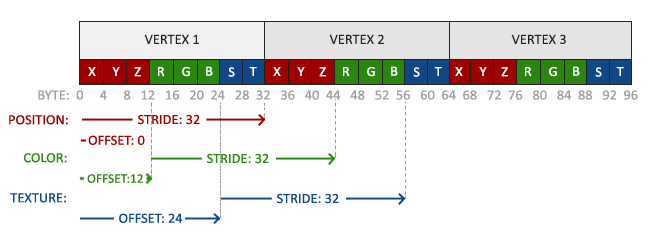
\includegraphics[width=\textwidth,height=\textheight,keepaspectratio]
    {resources/vertex_attribute_pointer_interleaved_textures.png}
    \caption{Vertex attribútumok elrendezése a memóriában\cite{vertexlayout}}
    \label{fig:vertexlayout}
\end{figure}

\subsection{IndexBuffer}
A primitve assembly során minden vertexet összekötünk egy bizonyos sorrendben, ezáltal megadva az alakzatunkat. Erre használhatunk egy úgynevezett \mintinline{cpp}{IndexBuffer}-t, ami megadja, hogy ez a folyamat milyen sorrendben történjen. Szimplán csak egy tömbre van szükségünk ami pozitív egész számokat tárol amik megmondják, hogy a vertexek milyen sorrendben lesznek összekötve és annak a hosszára.

\subsection{Shaderek}
Sokan amikor a shader szót először meghallják, rögtön arra gondolnak, hogy megvilágítás vagy árnyékolás. Valójában egy shader szimplán csak egy program, ami a videokártyán fut. Egy shader program létrehozásához csupán a forráskódjára és a típusára van szükségünk. Első lépésben létrehozunk egy shader-t a típusa alapján a \verb|glCreateShader()| metódussal, melyet egy pozitív egész szám fog azonosítani, OpenGL-ben ez az objektum azonosító. Beállítjuk neki a forráskódját a \verb|glShaderSource()| függvénnyel, majd lefordítjuk a \verb|glCompileShader()| metódussal. Ha a fordítás során valami hiba történik, akkor ezt ki tudjuk írni a felhasználó számára és ez alapján kijavíthatja a hibát a kódjában. Ha a shader sikeresen lefordult, akkor visszatérhetünk az azonosítójával.

Még nem vagyunk teljesen kész, a lefordított shadereket hozzá kell csatolnunk egy programhoz, majd ezt a programot linkelnünk. Itt is ugyanúgy  kiírathatjuk a hibaüzenetet, ha valami akadályba ütközik az API a linkelés során. Végső lépésben a programot validálhatjuk, majd törölhetjük a shadereket mert már nincs rájuk szükségünk és visszatérünk a program azonosítójával, ami az objektum \mintinline{cpp}{RendererID}-ja lesz. Ezt az azonosítót átadva a \mintinline{cpp}{glUseProgram(m_RendererID)} függvénynek a programot aktiválhatjuk.

\subsection{Uniformok}
A uniformok olyan globális GLSL változók, melyeket kézzel állíthatunk be kívülről és akár minden képkocka során frissíthetjük őket. Uniformok segítségével tudunk olyan információkat feltölteni a shaderbe, mint a képernyő felbontását, a kurzor pozícióját, az eltelt időt, és textúrákat samplerek formájában az azonosítójukon keresztül. Egy uniform beállításához három dologra van szükségünk, a shader program azonosítójára amihez szeretnénk a uniformot csatolni, egy string-re, amivel majd tudunk hivatkozni a uniformra a forráskódon belül, és az értékre, amit a uniformnak adni akarunk. Az alkalmazásban minden uniformot egy u\_ prefixel jelölök.

\begin{minted}
[bgcolor=lbcolor,showspaces=false,breaksymbolleft=,breaklines=true]
{cpp}
m_UniformManager.SetUniform1f(rendererId, 
                              "u_" + name + "Time",
                              glfwGetTime());
\end{minted}        

\subsection{Textúrák}

Képesek vagyunk minden shaderhez több darab textúrát is rendelni. A \mintinline{cpp}{Textures} konstruktora egy listát vár paraméterül, ami tartalmazza a használni kívánt textúrák elérési útját. A képek beolvasására használjuk az stb\_image kép kezelő könyvtárat, aminek a kép beolvasásához csak egy elérési útvonalra, néhány paraméterre és egy változóra van szüksége, amiben majd el tudja tárolni a kép adatait. 
Minden textúrát beolvasunk az stbi\_image könyvtár \mintinline{cpp}{stbi_load()} függvényével, a textúrák lehetnek például .jpg, .png, .bmp formátumú képek. Ez paraméterül vár egy elérési utat, két változót amibe beállítja a beolvasott textúra szélességét és magasságát, még egy változót, amibe a fájl színcsatornáinak a száma kerül és végül, hogy ebből hány csatornát szeretnénk megtartani.

Minden textúrához kérnünk kell egy azonosítót az API-tól, majd beállítani, hogy ez az azonosító egy textúrát jelöl.

\begin{minted}{cpp}
glGenTextures(1, &m_TextureIds[counter]);
\end{minted}

A textúráknak megadhatunk különböző paramétereket, hogy egyes esetekben miként kezelje a texúrák rajzolását. Például, hogy végezzen a textúrán akármilyen filterezést vagy átméretezés során inkább széthúzza a textúrát vagy megismételje azt.

Ezután pedig fel kell töltenünk a textúra adatait a grafikus memóriába.

\begin{minted}
[bgcolor=lbcolor,showspaces=false,breaksymbolleft=,breaklines=true]
{cpp}
 glTexImage2D(GL_TEXTURE_2D,
              0, GL_RGBA8,
              m_Width,
              m_Height,
              0, GL_RGBA,
              GL_UNSIGNED_BYTE,
              m_LocalBuffer);
\end{minted}

Utolsó lépés pedig, hogy a textúrához rendeljünk egy sampler típusú uniformot, amin keresztül majd a forráskódban tudunk rá hivatkozni.

\begin{minted}
[bgcolor=lbcolor,showspaces=false,breaksymbolleft=,breaklines=true]
{cpp}
 m_UniformManager.SetUniform1i(
    rendererId,
    samplerName.str(),
    counter);
\end{minted}

\*subsection{Az objektumok kapcsolatai}

Ezeket az objektumokat lényegében azért hoztuk létre, hogy a shaderekben adatokat tudjunk elérni. A vertex tömbökön keresztül a vertex kordinátákat, a textúrákon keresztül kép adatokokat. Az indexek sorrendje szerint összekötjük a vertexeket, a vertex shader alapján transzformáljuk őket, a fragmens shader szerint pedig színezzük a rajzolt alakzatokat. Az uniformokon pedig egyéb adatokat érhetünk el a shaderek forráskódjaiban.